
%%%%%%%%%%%%%%%%%%%%%%%%%%%%%%%%%%%%%%%%%%%%%%%%%%%%%%%%%%%%%%%%%
\documentclass[a4paper,abstracton]{scrartcl}

% author and affiliation block
\usepackage{authblk}
\renewcommand\Affilfont{\small}

% maths packages
\usepackage{mathtools}
\usepackage{amssymb}
\usepackage{bm}

% bibliography and referencing
\usepackage{natbib}
\bibliographystyle{apalike}
\usepackage{hyperref}
\usepackage{xcolor}
\definecolor{darkgreen}{RGB}{0,127,173}
\definecolor{darkblue}{RGB}{0,0,200}
\hypersetup{colorlinks, linkcolor={darkblue}, citecolor={darkgreen}, urlcolor={darkblue}}

% figures and graphics
\usepackage{graphicx}
\graphicspath{{figures/}}  % path to directory containing all figures
\usepackage{caption}  % allows subfigures
\usepackage{subcaption}  % allows subfigures

% layout and formatting
\allowdisplaybreaks  % allows page breaks within equations
\usepackage{multirow}  % table formatting

% macros
\newcommand{\F}{{\mathcal{F}}}
\newcommand{\M}{{\mathcal{M}}}
\newcommand{\U}{{\mathcal{U}}}
\newcommand{\X}{{\mathcal{X}}}
%%%%%%%%%%%%%%%%%%%%%%%%%%%%%%%%%%%%%%%%%%%%%%%%%%%%%%%%%%%%%%%%%


\begin{document}

\title{A faster exact method for solving the robust multi-mode resource-constrained project scheduling problem}

\author[1]{Matthew Bold\footnote{Corresponding author, email: m.bold1@lancaster.ac.uk}}
\author[2]{Marc Goerigk}

\affil[1]{STOR-i Centre for Doctoral Training, Lancaster University, Lancaster, UK}	
\affil[2]{Network and Data Science Management, University of Siegen, Siegen, Germany}	

\date{}

\maketitle

\begin{abstract}
\end{abstract}

\noindent\textbf{Keywords:} project scheduling; optimisation under uncertainty; robust optimisation; budgeted uncertainty

%%%%%%%%%%%%%%%%%%%%%%%%%%%%%%%%%%%%%%%%%%%%%%%%%%%%%%%%%%%%%%%%%%%%%%%%%

\section{Introduction}
The multi-mode resource-constrained project scheduling problem (MRCPSP) is a generalisation of the widely-studied resource-constrained project scheduling problem (RCPSP) to include multiple processing modes for each activity. The purpose of introducing activity processing modes is to model situations in which there is more than one way of executing project activities, with each option having its own duration and resource requirements. The MRCPSP consists selecting the processing modes and start times for a given set of activities, subject to a set of precedence constraints and limited resource availability, with the objective of minimising the overall project duration, known as the makespan.

The work in the paper extends the compact reformulation for the RCPSP developed by \cite{bold2021compact} for application to the MRCPSP. A computational study is presented comparing this approach against the Benders' decomposition approach used in \cite{balouka2021robust} for solving MRCPSP instances with uncertain activity durations. Note that the method used in \cite{balouka2021robust} is an extension of the approach used by \cite{bruni2017adjustable} to solve the RCPSP with uncertain activity durations.

* lit review *

\section{Problem description}

A project consists of a set of non-preemptive activities $V=\{0,1,\dots,n,n+1\}$, where 0 and $n+1$ denote the dummy source and sink activities respectively. Each activity $i\in V$ has a set of available processing modes given by $M_i=\{1,\dots,|M_i|\}$. We denote a particular choice of mode selections as $\bm{m}=(m_1,\dots,m_n)$, and the set of all possible mode selections by $\M\subseteq \mathbb{N}^n$. The nominal duration of activity $i$ when executed in mode $m_i\in M_i$ is given by $\hat{d}_{im_i}$, whilst its worst-case duration is given by $\bar{d}_{im_i}+\hat{d}_{im_i}$, where $\hat{d}_{im_i}$ is its maximum durational deviation. Each mode for activity $i$, $m_i\in M_i$, has an associated renewable resource requirement of $r_{im_ik}$ for each $k\in K$, where $K$ is the set of renewable resource types involved in the project. Each renewable resource $k\in K$ has an availability of $R_{k}$ at each time period in the project horizon. As well as resource constraints, the project is subject to a set of strict finish-to-start precedence constraints given by $E$, where $(i,j)\in E$ enforces that activity $i$ must finish before activity $j$ can begin. A project can be represented on a directed graph $G(V,E)$. Figure \ref{fig:mrcpsp_network} shows an example uncertain MRCPSP instance involving five non-dummy activities and a single renewable resource.

\begin{figure}[h]
	\centering
	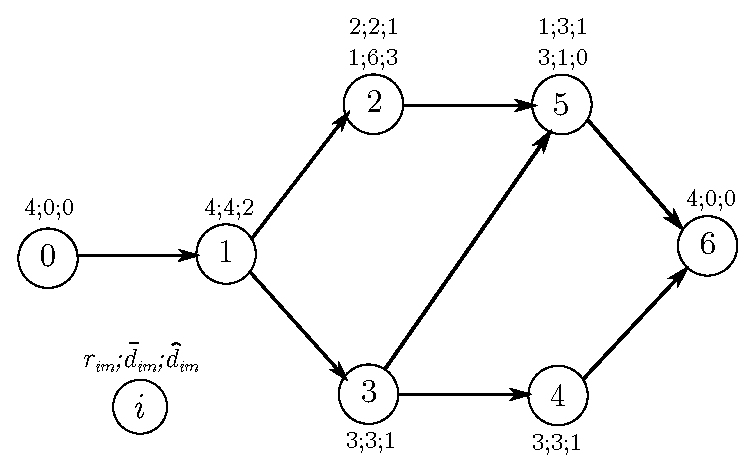
\includegraphics[scale=1]{mrcpsp_network.pdf}
	\caption{Example of an uncertain MRCPSP instance involving five non-dummy activities and a single renewable resource with an availability of 4. Activities 2 and 5 each have two available processing modes, whilst the other activities have only a single mode.}
	\label{fig:mrcpsp_network}
\end{figure}


For a given choice of processing modes for each activity $\bm{m}$, we assume that the activity durations lie somewhere in a budgeted uncertainty set of the form
$$\U_{\bm{m}}(\Gamma)=\Bigg\{\bm{d}\in\mathbb{R}_+^{|V|}:d_{im_i}=\bar{d}_{im_i}+\xi_i\hat{d}_{im_i},\,0\leq \xi_i \leq 1,\,\forall i\in V,\,\sum_{i\in V}\xi_i \leq \Gamma\Bigg\}.$$
Introduced by \cite{bertsimas2004price}, the motivation of the budgeted uncertainty set is to control the pessimism of the solution by introducing a robustness parameter $\Gamma$ to limit the number of jobs that can simultaneously achieve their worst-case durations. Observe that when $\Gamma=0$, each activity takes its nominal duration and the resulting problem is the deterministic MRCPSP. At the other extreme, when $\Gamma=n$, every activity takes its worst-case duration, in which case the uncertainty set becomes equivalent to an interval uncertainty set. In this case the problem can again be solved as a deterministic MRCPSP instance considering only worst-case durations.

For a given selection of activity modes $\bm{m}$, a forbidden set is defined to be any subset of activities $F_{\bm{m}}\subseteq V$ that are not precedence-related, such that $\sum_{i\in F_{\bm{m}}}r_{im_ik}>R_k$ for at least one resource $k\in K$. That is, a forbidden set is a collection of activities that cannot be executed in parallel only because of resource limitations.

Applying the main representation theorem of \cite{bartusch1988scheduling}, given a particular choice of activity modes $\bm{m}$, a solution to the MRCPSP can be defined by a set of additional precedences $X_{\bm{m}}\subseteq V^2\setminus E$ such that the extended precedence network $G(V,E\cup X_{\bm{m}})$ is acyclic and contains no forbidden sets. Such an extension to the project network is referred to as a \textit{sufficient selection}. 

Hence the two-stage robust MRCPSP under budgeted uncertainty, which we refer to as the robust MRCPSP, can be written as
\begin{align}
	& \min_{\bm{m}\in \M,\,X_{\bm{m}}\in \X_{\bm{m}}} \max_{\bm{d}\in\U_{\bm{m}}(\Gamma)} \min_{\bm{S}} S_{n+1}\label{eqn:robust_mrcpsp_1}\\
	& S_0 = 0\\
	& S_j - S_i \geq d_{im_i} \qquad \forall (i,j)\in E\cup X_{\bm{m}}\\
	& S_i \geq 0 \qquad \forall i\in V.\label{eqn:robust_mrcpsp_4}
\end{align}
This problem aims to selects activity modes and a corresponding sufficient selection in order to minimise the worst-case project makespan. 

\section{A compact reformulation}

We propose solving this problem using an extended version of the compact reformulation from \cite{bold2021compact}. The development of this formulation for the RCPSP involved a reformulation of the adversarial sub-problem of determining the worst-case distribution of $\Gamma$ delays among the project activities. The reformulated sub-problem took the form of a longest-path problem through an augmented project network. 

The derivation for the equivalent compact reformulation for the MRCPSP is more or less identical to the one presented in that paper for the RCPSP. We therefore omit its derivation here, and instead just present the resulting model.

\begin{align}
\min \ & S_{n+1,\Gamma}\label{eqn:compact1}\\
\text{s.t. } & S_{00}=0\label{eqn:compact2}\\
	     & S_{j\gamma} - S_{i\gamma} \geq \bar{d}_{im}x_{im} - N(1-y_{ij}) & \hspace{-5cm}\forall (i,j)\in V^2,\,\forall m\in M_i,\,\gamma=0,\dots,\Gamma\label{eqn:compact_bigM1}\\
	     & S_{j,\gamma+1} - S_{i\gamma} \geq (\bar{d}_{im} + \hat{d}_{im})x_{im} - N(1-y_{ij})\nonumber \\
	     &&\hspace{-5cm} \forall (i,j)\in V^2,\, m\in M_i,\,\gamma = 0,\dots,\Gamma-1\label{eqn:compact_bigM2}\\
	     & y_{ij}=1 & \forall (i,j) \in E\cup\{(n+1,n+1)\}\label{eqn:compact5}\\
	     & f_{ijk}\leq P_{ijk}y_{ij} & \hspace{-5cm}\forall (i,j)\in V^2,\,i\neq n+1,\,j\neq0,\, \forall k \in K\label{eqn:compact6}\\
	     & \sum_{i\in V\setminus\{n+1\}}f_{ijk}=\sum_{m\in M_j}r_{jmk}x_{jm} & \forall j \in V\setminus\{0\} ,\, \forall k\in K\label{eqn:compact7}\\
	     & \sum_{j\in V\setminus\{0\}}f_{ijk}=\sum_{m\in M_i}r_{imk}x_{im} & \forall i \in V\setminus\{n+1\},\,\forall k\in K\label{eqn:compact8}\\
	     & \sum_{m\in M_i}x_{im} = 1 & \forall i\in V\label{eqn:compact9}\\
	     & \sum_{m\in M_i}r^{\nu}_{imk}x_{im} \leq R^{\nu}_k & \forall i \in V,\,k\in K^{\nu}\\
	     & S_{i\gamma}\geq 0 &\forall i\in V,\,\gamma \in 0,\dots, \Gamma\label{eqn:compact10}\\
	     & f_{ijk}\geq 0 & \forall (i,j)\in V^2 ,\, \forall k \in K\label{eqn:compact11}\\
	     & y_{ij}\in\{0,1\} & \forall (i,j)\in V^2\label{eqn:compact12}\\
	     & x_{im}\in\{0,1\} & \forall i\in V,\,m\in M_i,
\end{align}
where $N=\sum_{i\in V}\max_{m\in M_i}(\bar{d}_{im}+\hat{d}_{im})$ is an upper bound on the minimum makespan, and $P_{ijk}=\min\{\max_{m\in M_i}r_{imk},\,\max_{m\in M_j} r_{jmk}\}$ is the maximum possible flow of resource $k$ from $i$ into $j$.

This formulation can be solved directly by a standard mathematical optimisation solver such as Gurobi or CPLEX.

\section{A Benders' decomposition approach}

In this section we outline a Benders' decomposition approach to solving the robust MRCPSP first presented in \cite{balouka2021robust}. As mentioned previously, this approach is based on the approach used to solve the robust RCPSP in \cite{bruni2017adjustable}.

The main idea behind this approach is to decompose the full problem into a two smaller problems: 1. a master problem that determines activity processing modes and resolves resource conflicts, and 2. a subproblem that takes the solution from the master problem and evaluates it by finding the worst-case makespan for the resulting network by solving a longest path problem. The solution to the master problem forms a lower bound to the optimal objective value of the original problem, whilst the solution to the subproblem provides an upper bound. These two problems are solved iteratively, with optimality cuts being added to the master problem each iteration based on the solution to the subproblem until the lower and upper bounds meet .

\subsection{The master problem}

The role of the master problem is to determine a choice of activity processing modes $\bm{m}$, as well as a sufficient selection $X_{\bm{m}}$ to resolve any resulting resource conflicts. The processing mode for each activity is determined by binary variables $x_{im}$. The $y_{ij}$ variables define a complete set of precedences between the project activities, either due to the original project precedence constraints, or due to the resolution of resource conflicts, i.e. $\{(i,j),\, i,j\in V:y_{ij}=1\}=T(E\cup X_{\bm{m}})$, where $T(E\cup X_{\bm{m}})$ is the transitive closure of the extended project precedence network. Resource flow variables $f_{ijk}$ track the amount of renewable resource $k$ that is transferred from activity $i$ to activity $j$ upon its completion. Finally, $s_i$ and $\phi_{ij}$ are additional variables used to define two relaxations of the subproblem to strengthen the master problem formulation. Using these variables, the master problem can be formulated as follows:  
\begin{align}
	& \min \eta\label{eqn:master_first}\\
	& y_{ij} = 1 \qquad \forall (i,j)\in E \label{eqn:master_y1}\\
	& y_{ij} + y_{ji} \leq 1 \qquad \forall i,j\in V,\, i<j\label{eqn:master_y2}\\
	& y_{ij} = y_{ip} + y_{p j} - 1 \qquad \forall i,j,p\in V,\,i\neq j\neq p\label{eqn:master_y3}\\
	& f_{ijk} \leq \min(r_{im_ik}, r_{jm_jk})\cdot y_{ij} + (1 - x_{i,m_i})(\bar{r}_{ijk} - \min(r_{im_ik}, r_{jm_jk}))\nonumber\\
	& & \hspace{-8cm} + (1 - x_{j,m_j})(\bar{r}_{ijk} - \min(r_{im_ik}, r_{jm_jk})) \nonumber \\
	& & \hspace{-10cm}\forall i\in V\setminus\{n+1\},\, j \in V\setminus\{0\},\, i\neq j,\,m_i\in M_i,\,m_j\in M_j,\,k\in K\label{eqn:master_f1}\\
	& \sum_{i\in V\setminus\{j,n+1\}}f_{ijk} = \sum_{m\in M_j}r_{jmk}x_{jm} \qquad \forall j \in V\setminus\{0\} ,\,k\in K\label{eqn:master_f2}\\
	& \sum_{j\in V\setminus\{0,i\}}f_{ijk} = \sum_{m\in M_i}r_{imk}x_{im} \qquad \forall i \in V\setminus\{n+1\} ,\,k\in K\label{eqn:master_f3}\\
	& \sum_{m\in M_i}x_{im} = 1\qquad \forall i \in V\label{eqn:master_x}\\
	& \sum_{m\in M_i}r^{\nu}_{imk}x_{im} \leq R^{\nu}_k \qquad \forall i\in V,\,k\in K^{\nu}\label{eqn:master_nonrenewable}\\
	& \eta \geq \lambda(x, y, M^{*\ell}) \qquad \forall \ell=0,\dots,t-1\label{eqn:master_cuts}\\
	& s_j - s_i \geq \bar{d}_{im} - N(1-y_{ij}) - N(1-x_{im}) \qquad \forall i,j\in V,\, i\neq j,\,m\in M_i\label{eqn:master_relaxation1_1}\\
	& \eta \geq s_{n+1}\label{eqn:master_relaxation1_2}\\
	& \eta \geq \sum_{i \in V}\sum_{j\in V}\Big(\min_{m\in M_i}\bar{d}_{im}\Big)\phi_{ij}\label{eqn:master_relaxation2_1}\\
	& \sum_{j\in V}\phi_{ji} = \sum_{j\in V}\phi_{ij} \qquad \forall i \in V\setminus\{0,n+1\}\\
	& \sum_{j\in V}\phi_{0j} = 1\\
	& \sum_{j\in V}\phi_{j,n+1} = 1\\
	& \phi_{ij} \leq y_{ij} \qquad \forall i,j\in V,\,i\neq j\label{eqn:master_relaxation2_5}\\
	& y_{ij} \in\{0,1\} \qquad \forall i,j\in V,\,i\neq j\\
	& x_{im} \in \{0,1\} \qquad \forall i \in V,\, m\in M_i\\
	& f_{ijk} \geq 0 \qquad \forall i\in V\setminus\{n+1\},\,j\in V\setminus\{0\},\,i\neq j,\,k\in K\\
	& s_i \geq 0 \qquad \forall i\in V\\
	& \phi_{ij} \geq 0 \qquad \forall i,j\in V \label{eqn:master_last}
\end{align}
where $\bar{r}_{ijk}=\max(\max_{m\in M_i}r_{imk},\,\max_{m\in M_j}r_{jmk})$ is the maximum usage of resource $k\in K$ by either activity $i$ or $j$, and as before, $N=\sum_{i\in V}\max_{m\in M_i}(\bar{d}_{im}+\hat{d}_{im})$ is an upper bound on the minimum makespan.

The solution to he optimal objective value of the master problem (\ref{eqn:master_first})-(\ref{eqn:master_last}), denoted by $\eta^*$, forms a lower bound to the original robust MRCPSP problem. Note that for the first iteration, the solution to the master problem corresponds to an optimal solution to the MRCPSP with nominal activity durations. 

The original project precedence relations are captured by constraint (\ref{eqn:master_y1}). Constraints (\ref{eqn:master_y2}) and (\ref{eqn:master_y3}) ensure that the extended network is transitive and acyclic. Constraints (\ref{eqn:master_f1}) prevents the flow of resource from $i$ to $j$ from exceeding either the amount that becomes available from the completion of $i$, or the amount that is required by $j$, accounting for their selected modes. Constraints (\ref{eqn:master_f2}) and (\ref{eqn:master_f3}) ensure that each activity receives the amount of each renewable resource that it requires. Constraints (\ref{eqn:master_x}) allows only one processing mode to be selected for each activity. Non-renewable resource constraints are defined by (\ref{eqn:master_nonrenewable}). Constraints (\ref{eqn:master_cuts}) define the optimality cuts generated at each of the previous iterations. These cuts are explained in greater detail in Section \ref{section:optimality_cuts}.

In line with \cite{bruni2017adjustable} and \cite{balouka2021robust}, two relaxations of the subproblem have been included in the master problem in order to strengthen it. The first relaxation is implemented through constraints (\ref{eqn:master_relaxation1_1}) and (\ref{eqn:master_relaxation1_2}). These simply enforce the extended precedence relationships using nominal activity durations for each processing mode. The second relaxation is captured by constraints (\ref{eqn:master_relaxation2_1})-(\ref{eqn:master_relaxation2_5}), which use flow variables $\phi_{ij}$ to form a longest-path problem through the extended project network using minimal activity durations.

\subsection{The subproblem}
 
The subproblem at iteration $t$ considers the worst-case makespan for the mode choices and sufficient selection from the master problem at iteration $t$, denoted by $\bm{m}^{*t}$ and $X_{\bm{m}^{*t}}$ respectively. This is done by solving an uncertain longest-path problem through the extended project network, where activity durations lie in the budgeted uncertainty set $\U_{\bm{m}^{*t}}(\Gamma)$. This problem can be formulated as 
\begin{align}
V^{*t} = &\max \sum_{(i,j)\in T(E\cup X_{\bm{m}^{*t}})} \bar{d}_{im^{*t}_i}\alpha_{ij} + \hat{d}_{im^{*t}_i}w_{ij}\\
	& \sum_{(i,n+1)\in T(E\cup X_{\bm{m}^{*t}})} \alpha_{i,n+1} = 1\\
	& \sum_{(0,i)\in T(E\cup X_{\bm{m}^{*t}})} \alpha_{0,i} = 1\\
	& \sum_{(i,j)\in T(E\cup X_{\bm{m}^{*t}})} \alpha_{ij} - \sum_{(j,i)\in T(E\cup X_{\bm{m}^{*t}})} \alpha_{ji} = 0 \qquad \forall i \in V\setminus\{0,n+1\}\\
	& w_{ij} \leq \xi_i \qquad \forall (i,j)\in T(E\cup X_{\bm{m}^{*t}})\\
	& w_{ij} \leq \alpha_{ij} \qquad \forall (i,j)\in T(E\cup X_{\bm{m}^{*t}})\\
	& \sum_{i\in V}\xi_i \leq \Gamma\\
	& \alpha_{ij}\in \{0,1\} \qquad \forall (i,j)\in T(E\cup X_{\bm{m}^{*t}})\\
	& w_{ij}\geq 0 \qquad \forall (i,j)\in T(E\cup X_{\bm{m}^{*t}})\\
	& 0\leq \xi_i \leq 1 \qquad \forall i\in V
\end{align}

Variables $\alpha_{ij}$ define the longest path through the network. This path, which we denote as $\pi^{*t}=\{(i,j),\,i,j\in V:\alpha_{ij}=1\}$ has length $V^{*t}$. Variables $\xi_i$ are the activity delay variables, whilst $w_{ij}$ are used to linearise the formulation.

\subsection{Optimality cuts} \label{section:optimality_cuts}

Following the solution to the subproblem, a valid cut is generated and added to the master problem for the next iteration. This cut simply forces an alternative solution in the master problem if it is to achieve a better objective value in the next iteration. 

Given the current best lower bound for the original problem $LB$, the mode selection from the master problem $\bm{m}^{*t}$, and the optimal objective value of the subproblem $V^{*t}$, the cut at iteration $t$ can be written as
\begin{align}
	& \eta \geq (V^{*t} - LB)\cdot\sum_{(i,j)\in \pi^{*t}}\bigg(1/3 (y_{ij} + x_{i,m_i^{*t}} + x_{j,m_j^{*t}}) - (3 - y_{ij} - x_{i,m_i^{*t}} - x_{j,m_j^{*t}})\bigg) & \nonumber \\
	& \hspace{8.1cm} - (V^{*t} - LB)\cdot(|\pi^{*t}|-1) + LB,\label{eqn:benders_cut}
\end{align}

\cite{balouka2021robust} show that this constraint is a valid optimality cut for the problem, and that the number of these cuts that need to be added to the master problem before finding an optimal solution is finite.

Before presenting a small example of the Benders' decomposition approach in the following subsection, we show an overview of the solution method in /ref. 

\subsection{Example}

\section{Computational experiments and results}
 
In this section we compare results from solving the compact reformulation with results from solving the Benders' decomposition approach. A complete set of the raw results used to generate the tables and plots presented here, in addition to the source code used to implement these experiments, can be found at \url{https://github.com/boldm1/robust-mrcpsp}.

The instances used in this computational study have been created using the deterministic $j10$, and $j20$ MRCPSP instances from the PSPLIB (\cite{kolisch1997psplib}, \url{https://www.om-db.wi.tum.de/psplib/}). The $j10$ set contains a total of 536 instances each involving 10 activities, and the $j20$ set contains a total of 554 instances each involving 20 activities. We introduce uncertainty into these deterministic instances by setting the maximum deviation of the duration for each activity to be $\hat{d}_{im}=\lfloor0.7\times \bar{d}_{im}\rfloor$ for each mode $m\in M_i$. We then solve each instance for a range of robustness levels $\Gamma$. In particular we solve the $j10$ instances for $\Gamma\in\{0,3,5,7\}$ and the $j20$ instances for $\Gamma\in\{0,5,10,15\}$. 

Both the compact reformulation and Benders' decomposition approach were implemented in Python 3.9.2 and solved using Gurobi 9.0.1 running on a single core of a 2.30 GHz Intel Xeon CPU. A time limit of 2 hours per instance was imposed on each of the solution methods.

Table \ref{table:benders_vs_compact} reports the percentage of instances solved to optimality (\textit{\%sol.}), the average optimality gap (in percent) over instances for which a feasible solution was found (\textit{gap}), and the average solution time (\textit{sol. time}) across the two instance sets and different choices of $\Gamma$, for both the Benders' decomposition approach and the compact reformulation. Note that if no optimal solution was found within the time limit by one of the solution methods, the solution time was recorded as the time limit value of 7200 seconds. Additionally, for the Benders' approach, the average number of iterations (\textit{it.}) and the average time per iteration (\textit{it. time}) are also reported. The average of these values across the different values for $\Gamma$ are also provided for each instance set.

\begin{table}[h]
\centering
\small  % font size
{\renewcommand{\arraystretch}{1.2}  % vertical padding
\begin{tabular}{lrrrrrrrrrrrr}
		     \hline \hline
		     &      & & \multicolumn{5}{c}{Benders'}                                       & & \multicolumn{3}{c}{Compact reformulation} \\
		     \cline{4-8} \cline{10-12}
		     & $\Gamma$ & & \textit{\%sol.} & \textit{gap} & \textit{its.} & \textit{it. time} & \textit{sol. time} & & \textit{\%sol.}   & \textit{gap}   & \textit{sol. time}   \\
		     \hline
	\multirow{4}{*}{$j10$} & 0    & & 99.6     & 0.00     & 1            & 73.6          & 100.4        & & 100.00     & 0.00       & 1.8             \\
			       & 3    & & 75.0     & 5.23     & 48           & 64.1          & 2065.6       & & 100.00     & 0.00       & 5.0             \\
			       & 5    & & 72.8     & 6.53     & 53           & 67.9          & 2234.5       & & 100.00     & 0.00       & 4.6             \\
			       & 7    & & 71.8     & 6.75     & 54           & 68.1          & 2278.4       & & 100.00     & 0.00       & 6.5             \\
		     \cline{4-8} \cline{10-12}
			       &      & & 79.8	   & 4.63     & 39.4	     & 68.4 	     & 1669.7	    & & 100.00     & 0.00	& 4.47 		  \\
		     \hline
	\multirow{4}{*}{$j20$} & 0    & & 80.8     & 0.00     & 1            & 123.5         & 1484.7       & & 89.4       & 1.92       & 941.9           \\
			       & 5    & & 39.6     & 10.91    & 173          & 124.8         & 5181.7       & & 88.4       & 1.91       & 1061.3          \\
			       & 10   & & 36.8     & 12.31    & 178          & 126.6         & 5406.2       & & 87.7       & 2.63       & 1138.4          \\
			       & 15   & & 36.8     & 12.48    & 177          & 135.2         & 5415.8       & & 86.0       & 2.96       & 1279.8          \\
		     \cline{4-8} \cline{10-12}
			       &      & & 48.5	   & 8.93     & 132.5	     & 127.5	     & 4372.1       & & 87.9       & 2.36       & 1105.4          \\
		     \hline \hline
\end{tabular}
}
\caption{Comparison of the Benders' decomposition approach and the compact reformulation across the $j10$ and $j20$ instance sets and the different values of $\Gamma$.}
\label{table:benders_vs_compact}
\end{table}

\begin{figure}[htb]
	\makebox[\textwidth][c]{
	\begin{subfigure}[t]{.65\textwidth}
		\centering
		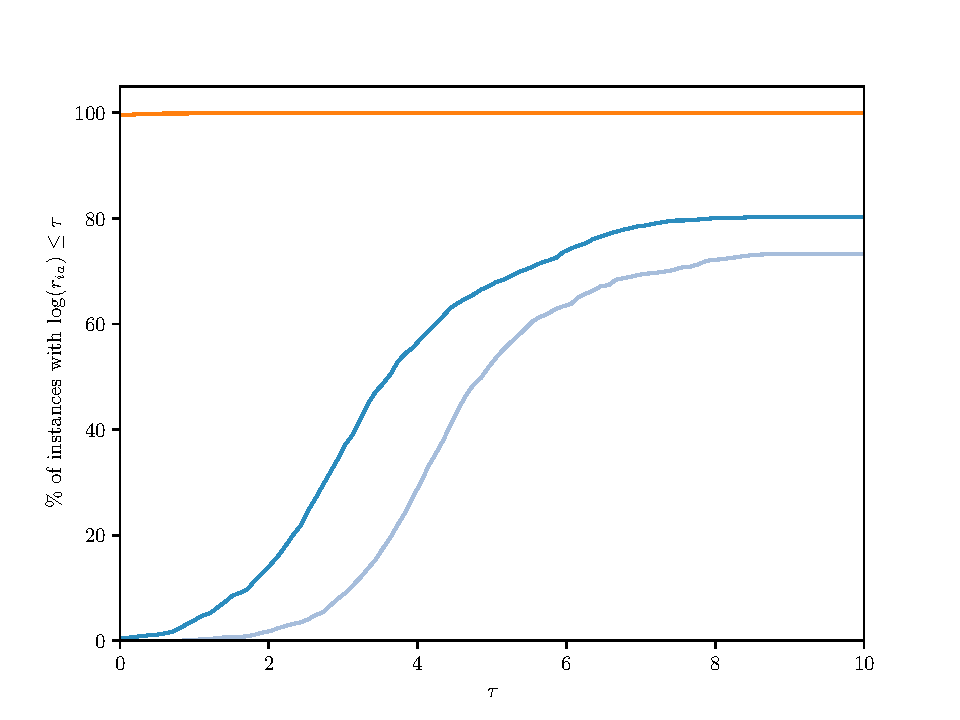
\includegraphics[width=1.05\textwidth]{j10_performance_profile.pdf}
		\caption{Performance profile of relative solution times.}\label{fig:j10_performance_profile}
	\end{subfigure}%
	\begin{subfigure}[t]{.65\textwidth}
		\centering
		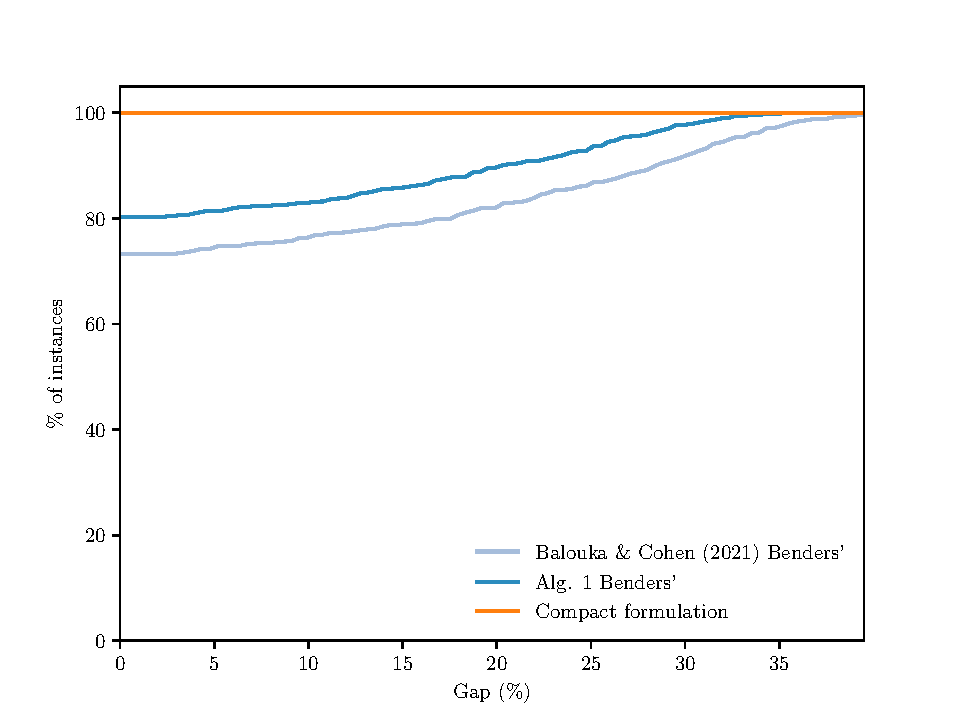
\includegraphics[width=1.05\textwidth]{j10_gaps.pdf}
		\caption{Percentage of instances solved to within given gap of optimality within the two-hour time limit.}\label{fig:j10_gaps}
	\end{subfigure}
	}
	\caption{Comparison of Benders' approach and compact reformulation over instances in the j10 set.}
	\label{fig:j10_plots}
\end{figure}

\begin{figure}[htb]
	\makebox[\textwidth][c]{
	\begin{subfigure}[t]{.65\textwidth}
		\centering
		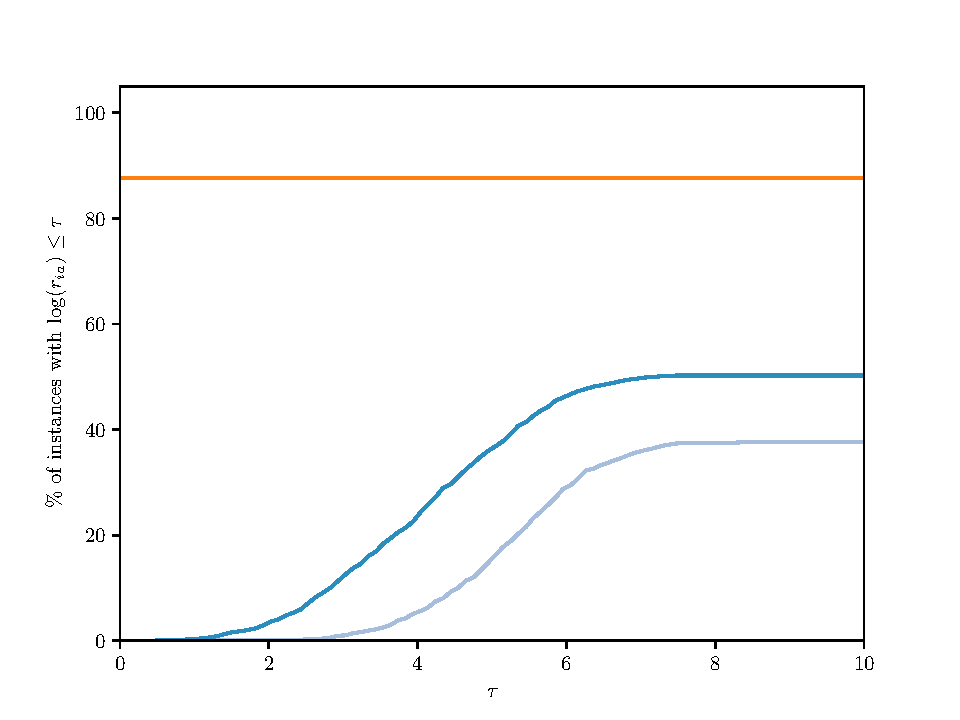
\includegraphics[width=1.05\textwidth]{j20_performance_profile.pdf}
		\caption{Performance profile of relative solution times.}\label{fig:j20_performance_profile}
	\end{subfigure}%
	\begin{subfigure}[t]{.65\textwidth}
		\centering
		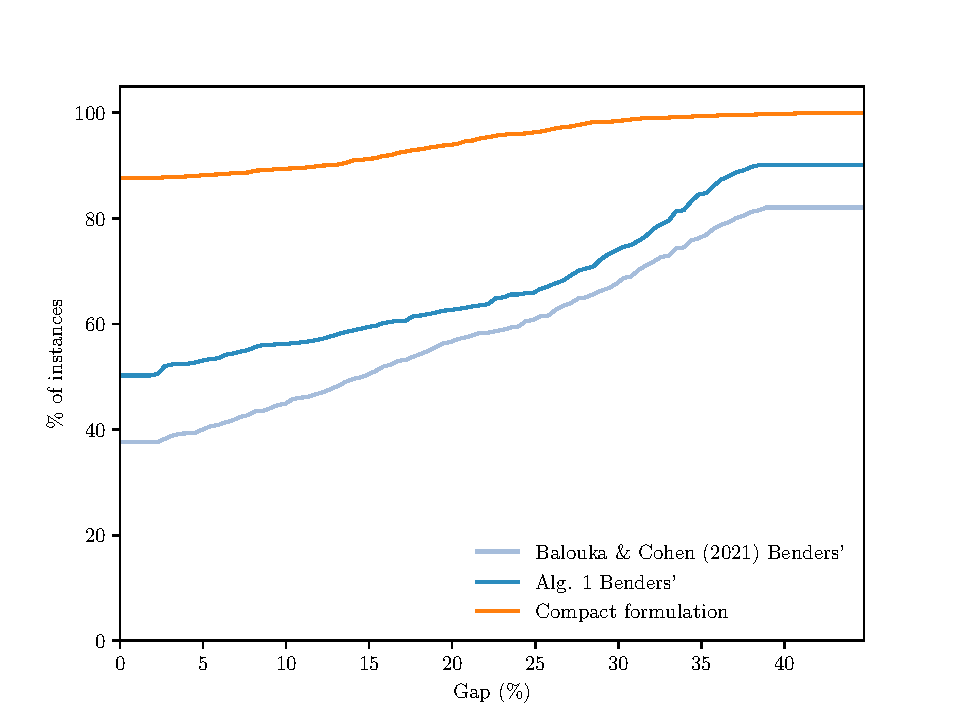
\includegraphics[width=1.05\textwidth]{j20_gaps.pdf}
		\caption{Percentage of instances solved to within given gap of optimality within the two-hour time limit.}\label{fig:j20_gaps}
	\end{subfigure}
	}
	\caption{Comparison of Benders' approach and compact reformulation over instances in the j20 set.}
	\label{fig:j20_plots}
\end{figure}

\section{Conclusions}


\section*{Acknowledgements}

The authors are grateful for the support of the EPSRC-funded (EP/L015692/1) STOR-i Centre for Doctoral Training.

\bibliography{paper}

\end{document}

